% !TeX root = ../../progress-sem1.tex
% Appendix: high-fidelity screens moved out of section 3.5 (committee comment).
% Screens are exported from the Figma file "Hi-Fidelity Wireframe", page "[REFERENCE THIS PAGE] Hi-fi v2";
% file names in figures/ch3-methodology/ui/ start with the hi-fi screen number.
\label{app:ui-screens}
\thaijustify{
  ภาคผนวกนี้รวบรวมหน้าจอ high-fidelity prototype ที่ออกแบบด้วย Figma แยกตามกลุ่มผู้ใช้ รายละเอียดของแต่ละหน้าจออยู่ในหัวข้อ~\ref{sec:ui-prototype}
}
\begin{figure}[H]
  \centering
  \subfloat[10 Projects]{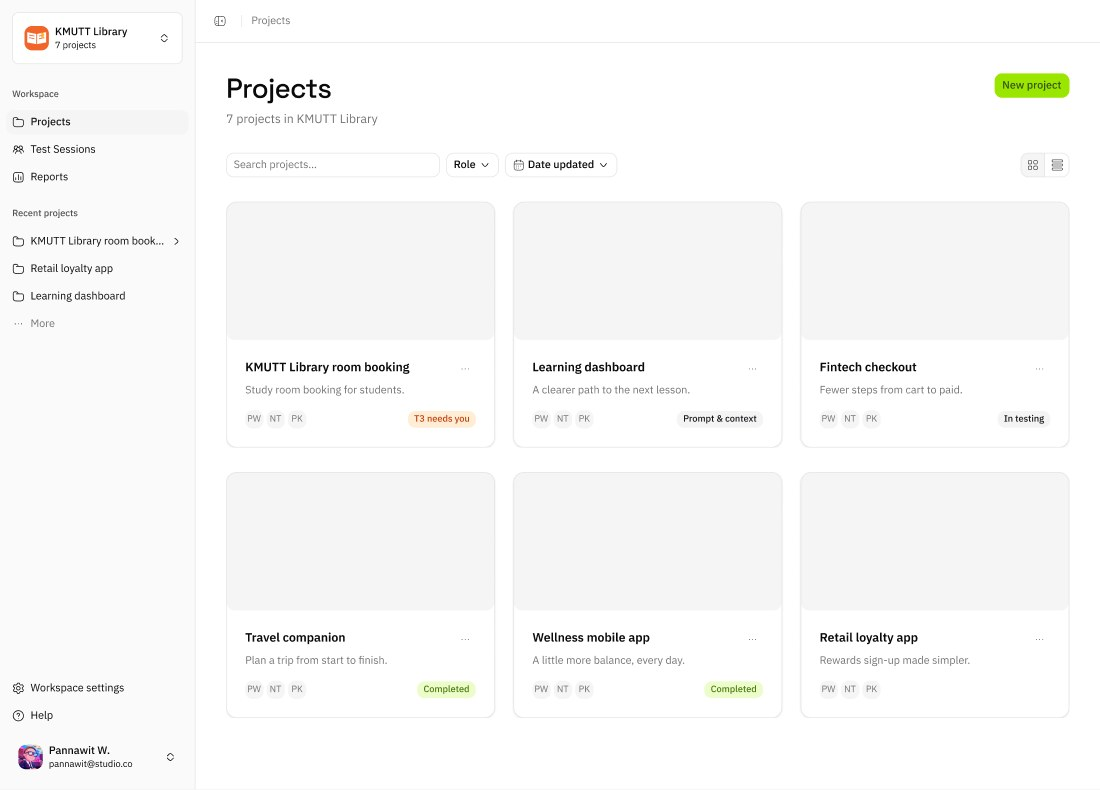
\includegraphics[width=0.48\linewidth,height=5.6cm,keepaspectratio]{figures/ch3-methodology/ui/d10-projects.jpg}}\hfill
  \subfloat[12 Design intent]{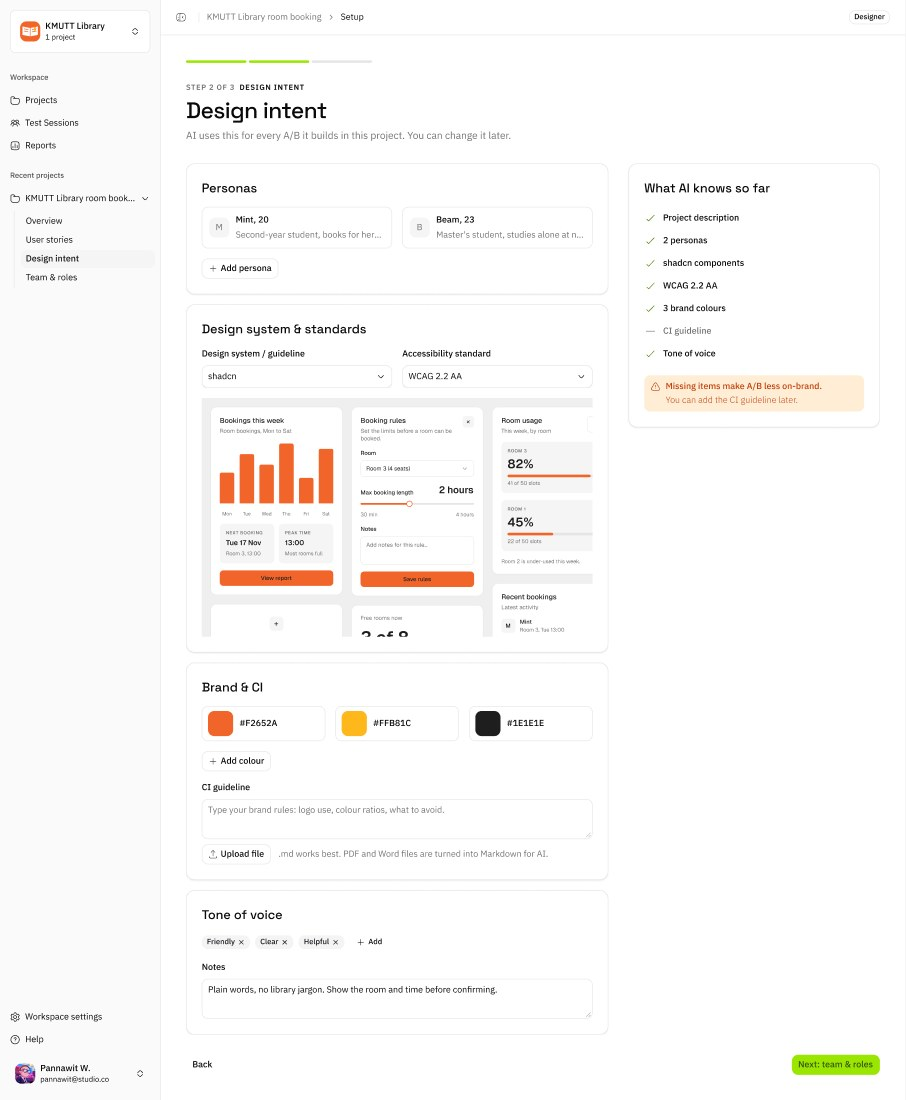
\includegraphics[width=0.48\linewidth,height=5.6cm,keepaspectratio]{figures/ch3-methodology/ui/d12-design-intent.jpg}}\\
  \subfloat[15 User story และ problem statement]{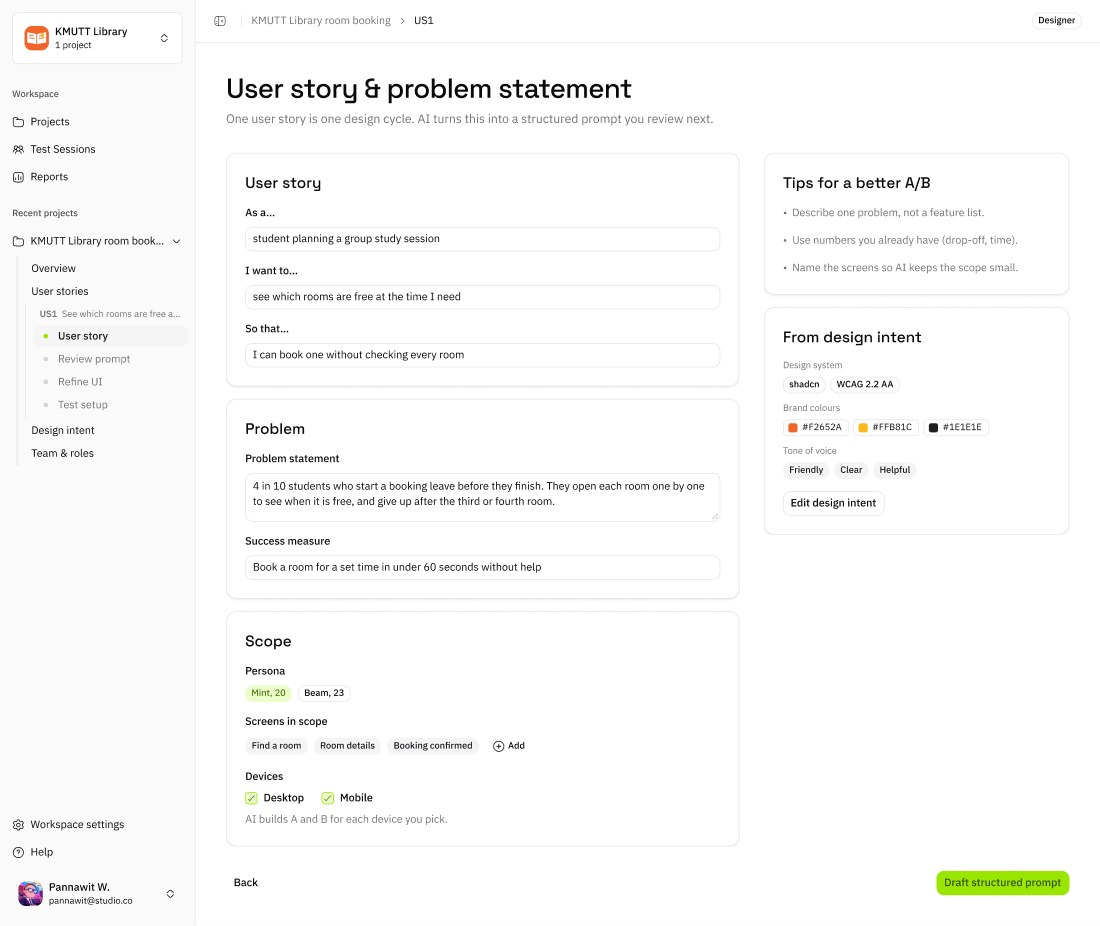
\includegraphics[width=0.48\linewidth,height=5.6cm,keepaspectratio]{figures/ch3-methodology/ui/d15-user-story.jpg}}\hfill
  \subfloat[16 Review structured prompt]{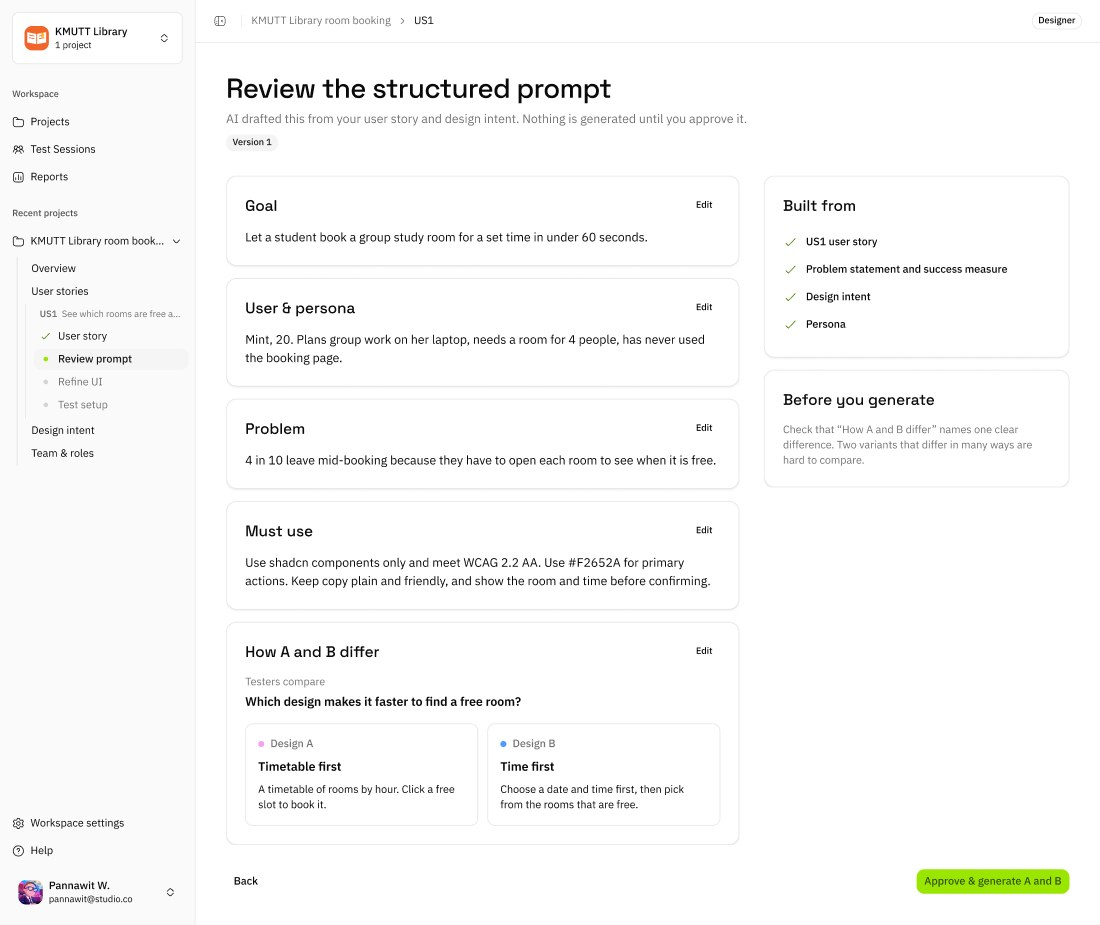
\includegraphics[width=0.48\linewidth,height=5.6cm,keepaspectratio]{figures/ch3-methodology/ui/d16-review-prompt.jpg}}\\
  \subfloat[17 Generating A/B]{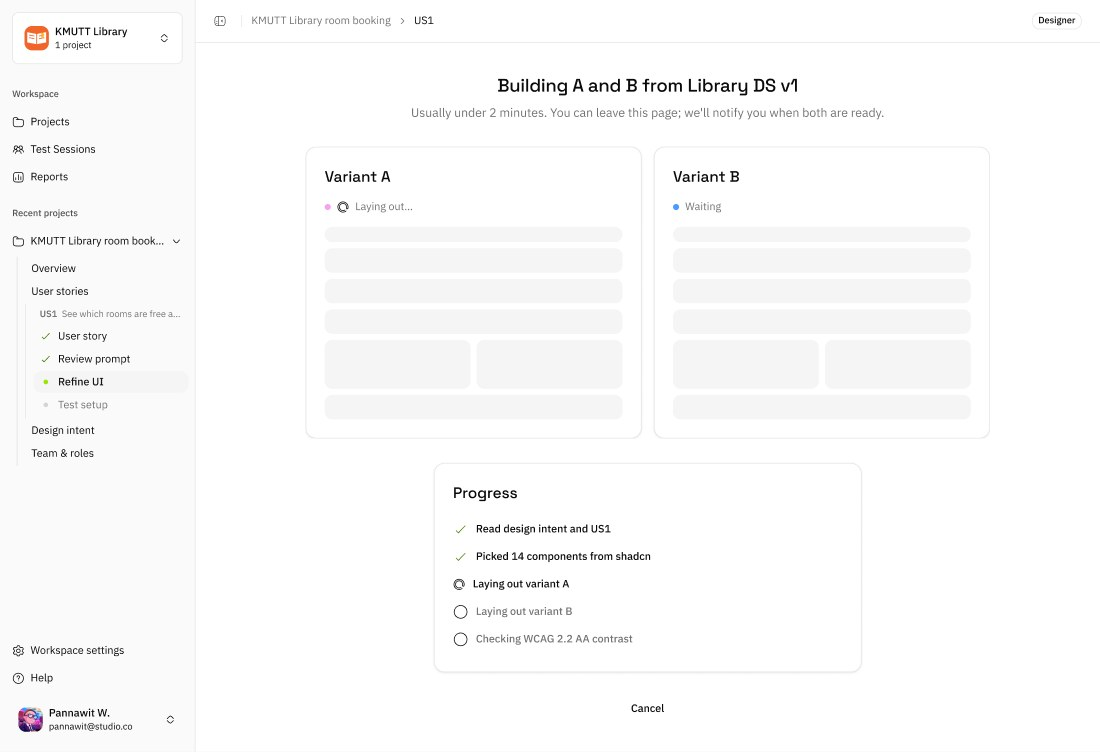
\includegraphics[width=0.48\linewidth,height=5.6cm,keepaspectratio]{figures/ch3-methodology/ui/d17-generating.jpg}}\hfill
  \subfloat[18 Refine A/B]{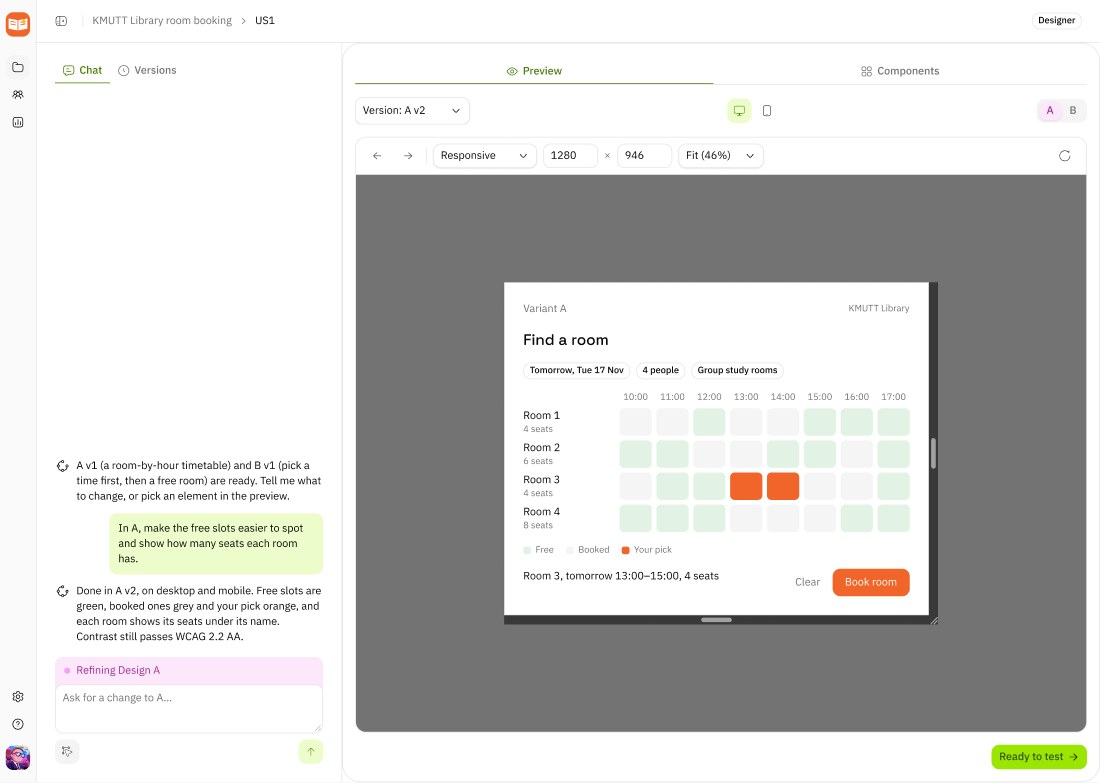
\includegraphics[width=0.48\linewidth,height=5.6cm,keepaspectratio]{figures/ch3-methodology/ui/d18-refine.jpg}}\\
  \caption{Prototype ของ Designer: การตั้งค่าโปรเจกต์และการสร้าง UI ด้วย AI}
  \label{fig:ui-designer-cycle}
\end{figure}
\begin{figure}[H]
  \centering
  \subfloat[19 Test setup]{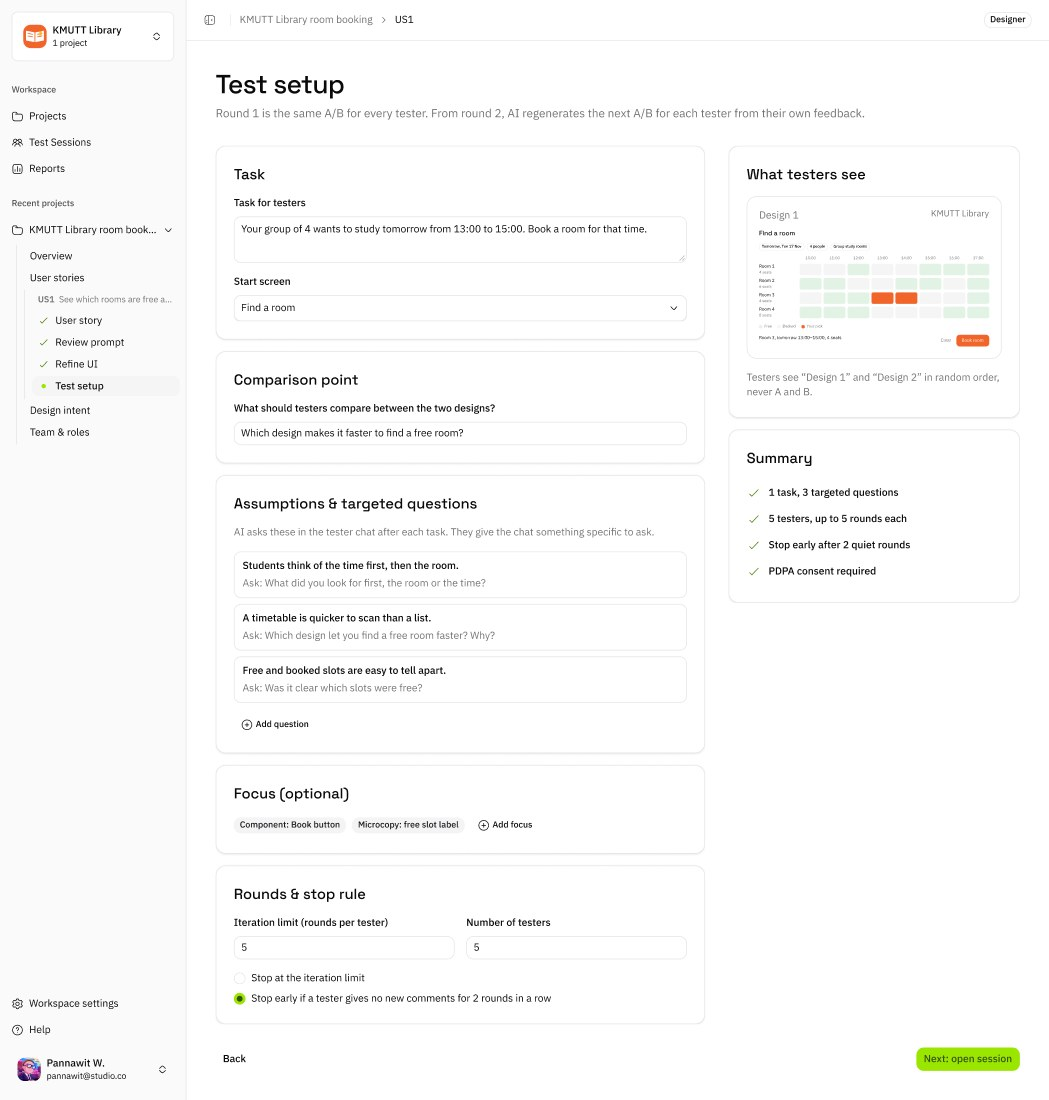
\includegraphics[width=0.48\linewidth,height=5.6cm,keepaspectratio]{figures/ch3-methodology/ui/d19-test-setup.jpg}}\hfill
  \subfloat[21 Monitor testers]{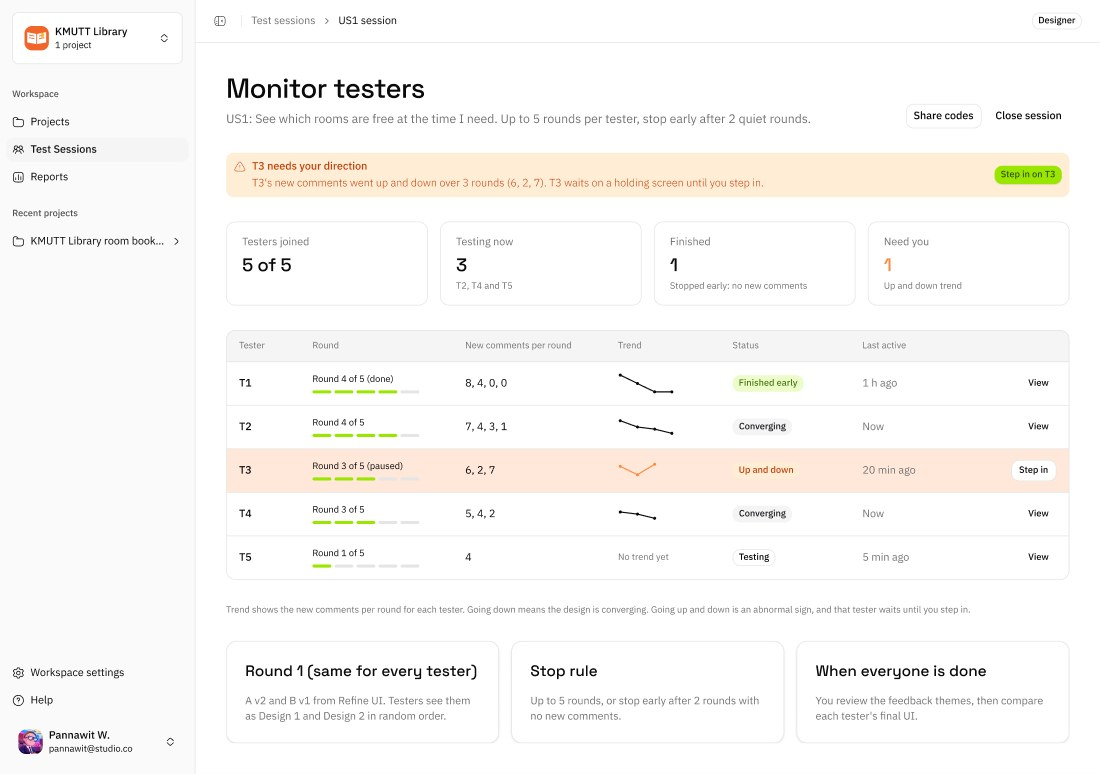
\includegraphics[width=0.48\linewidth,height=5.6cm,keepaspectratio]{figures/ch3-methodology/ui/d21-monitor.jpg}}\\
  \subfloat[23 Review feedback themes]{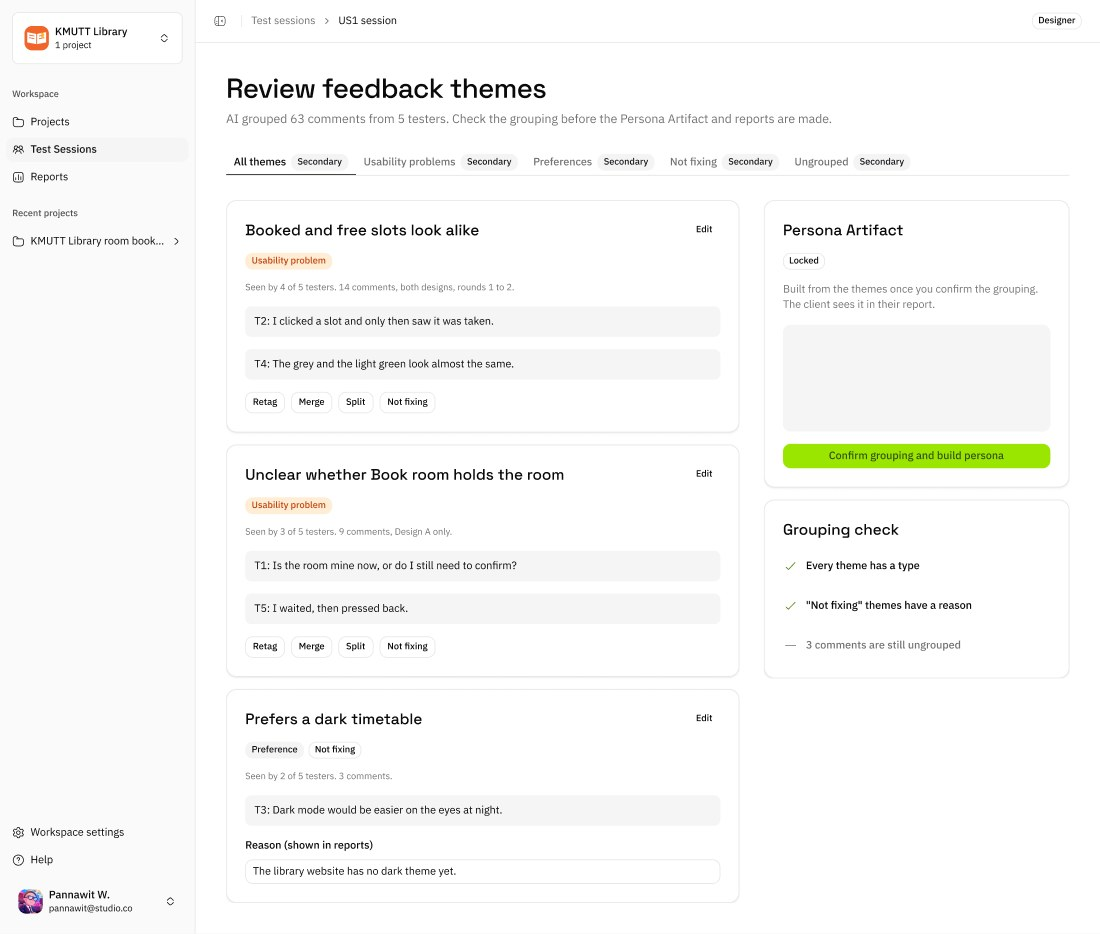
\includegraphics[width=0.48\linewidth,height=5.6cm,keepaspectratio]{figures/ch3-methodology/ui/d23-themes.jpg}}\hfill
  \subfloat[25 Role reports]{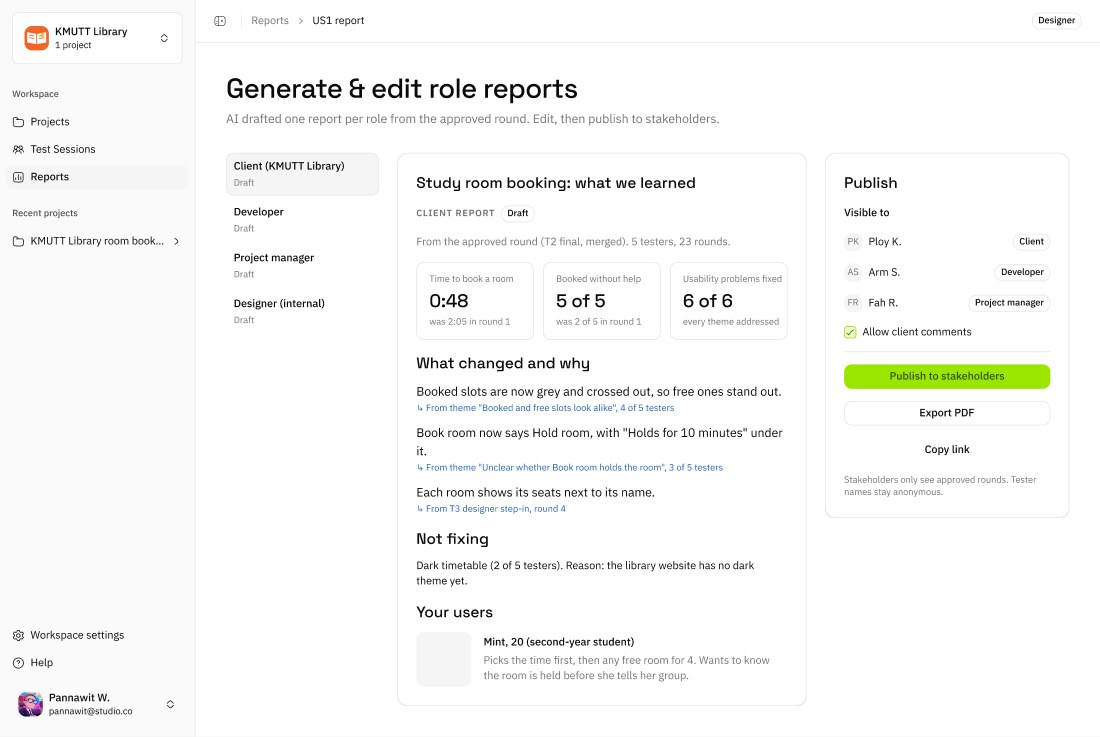
\includegraphics[width=0.48\linewidth,height=5.6cm,keepaspectratio]{figures/ch3-methodology/ui/d25-role-reports.jpg}}\\
  \caption{Prototype ของ Designer: การทดสอบ การวิเคราะห์ข้อเสนอแนะ และรายงาน}
  \label{fig:ui-designer-testing}
\end{figure}
\begin{figure}[H]
  \centering
  \subfloat[27 Consent (PDPA)]{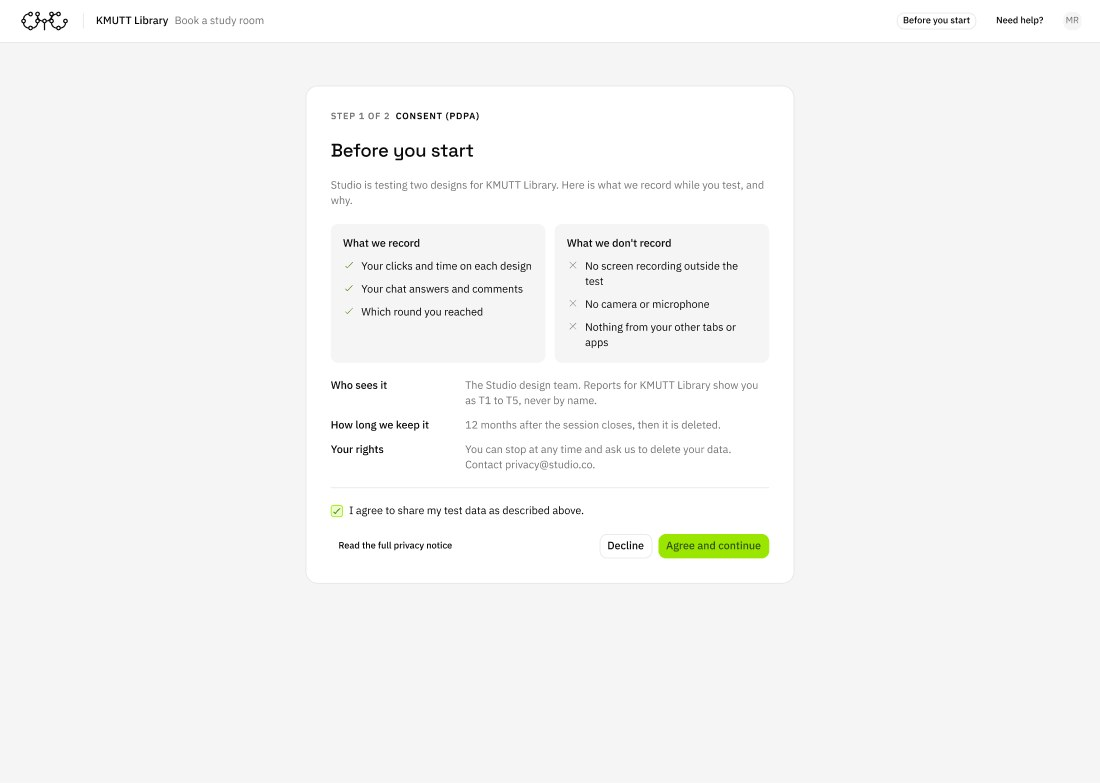
\includegraphics[width=0.48\linewidth,height=5.6cm,keepaspectratio]{figures/ch3-methodology/ui/t27-consent.jpg}}\hfill
  \subfloat[29 Task on Design 1 and 2]{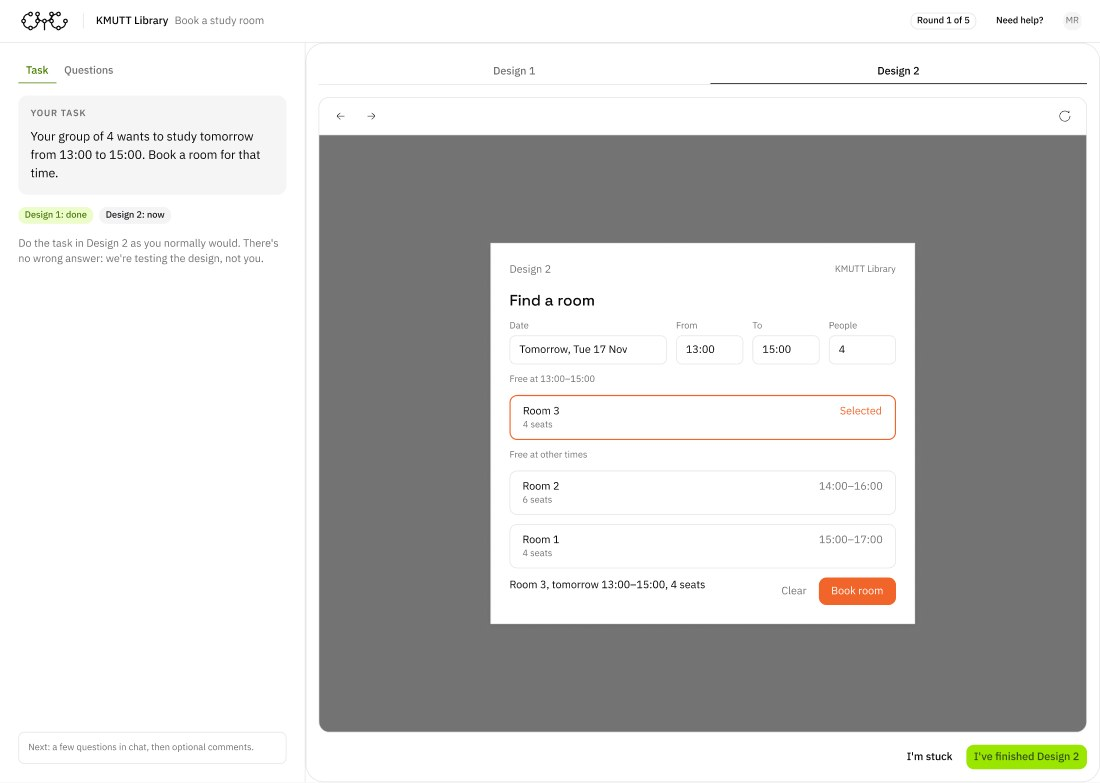
\includegraphics[width=0.48\linewidth,height=5.6cm,keepaspectratio]{figures/ch3-methodology/ui/t29-task.jpg}}\\
  \subfloat[30 Chat feedback]{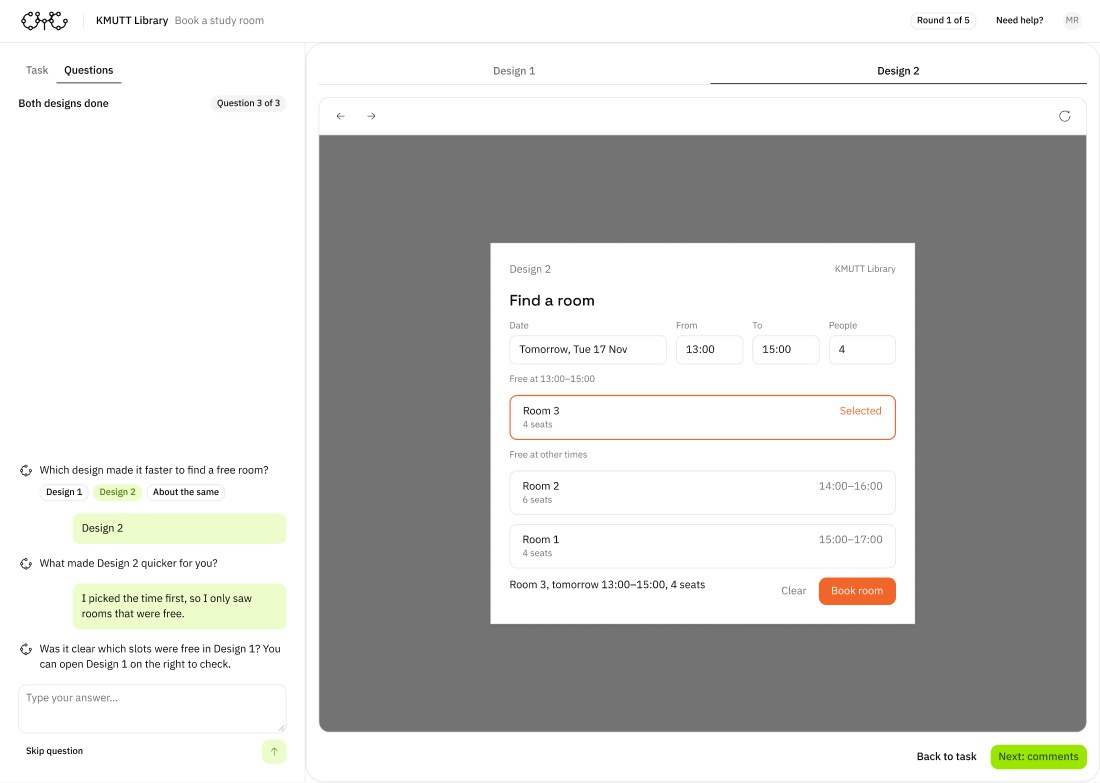
\includegraphics[width=0.48\linewidth,height=5.6cm,keepaspectratio]{figures/ch3-methodology/ui/t30-chat.jpg}}\hfill
  \subfloat[31 Pin a part and comment]{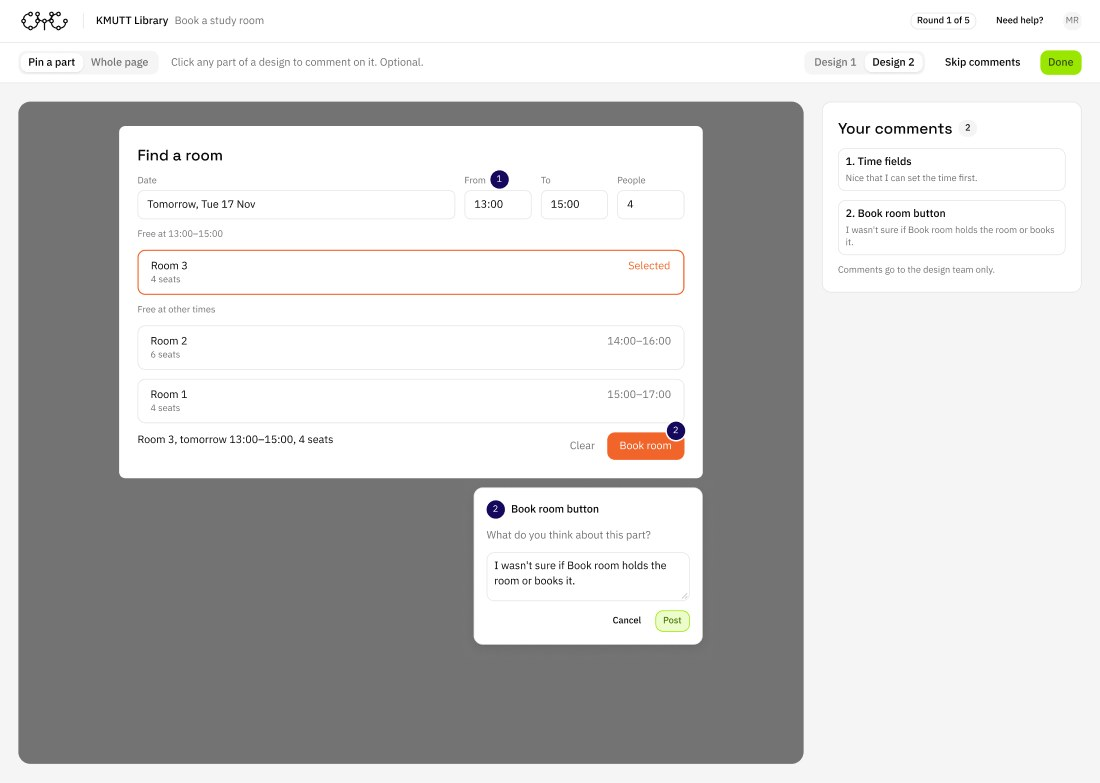
\includegraphics[width=0.48\linewidth,height=5.6cm,keepaspectratio]{figures/ch3-methodology/ui/t31-pin.jpg}}\\
  \caption{Prototype ของ Usability Tester}
  \label{fig:ui-tester}
\end{figure}
\begin{figure}[H]
  \centering
  \subfloat[37 Client report]{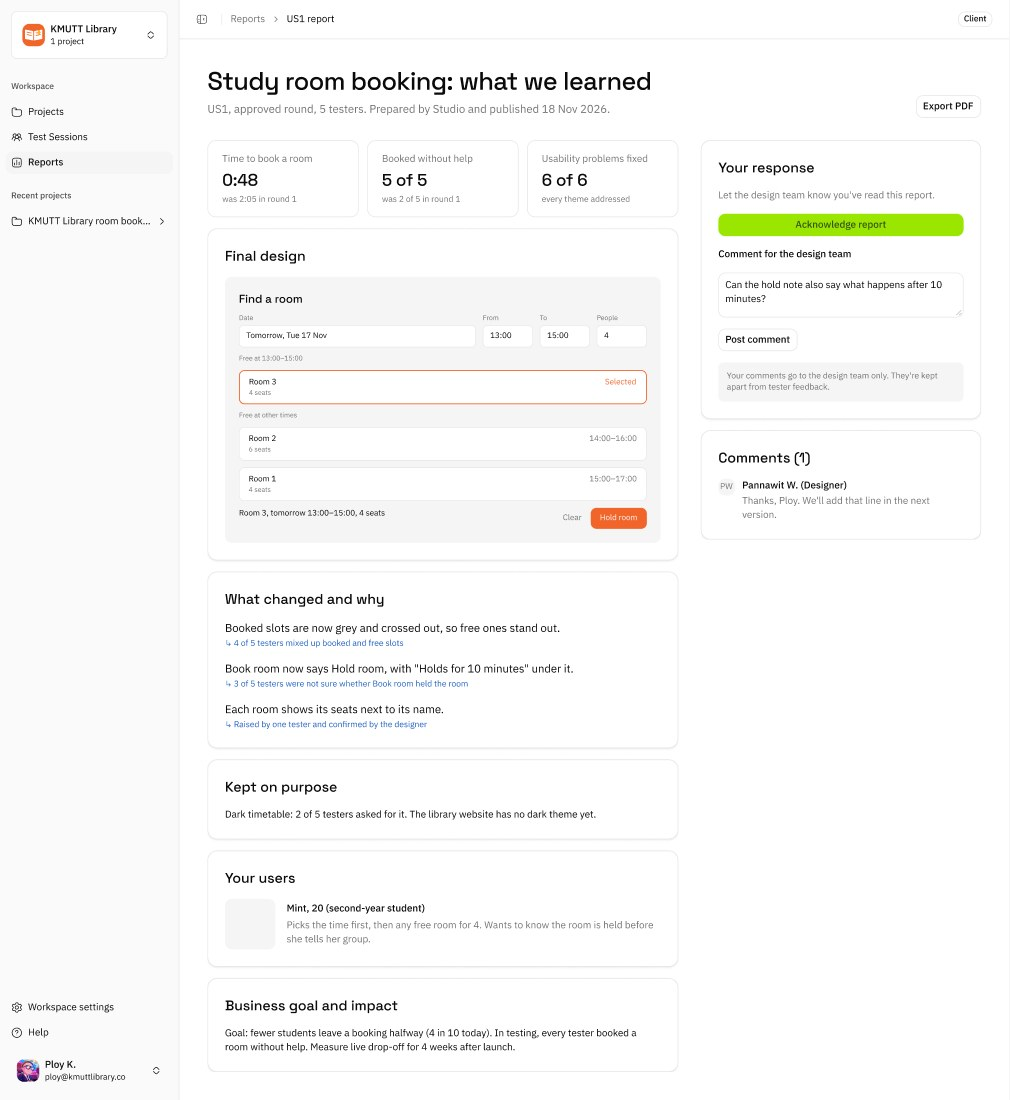
\includegraphics[width=0.48\linewidth,height=7cm,keepaspectratio]{figures/ch3-methodology/ui/s37-client.jpg}}\hfill
  \subfloat[38 Developer handoff]{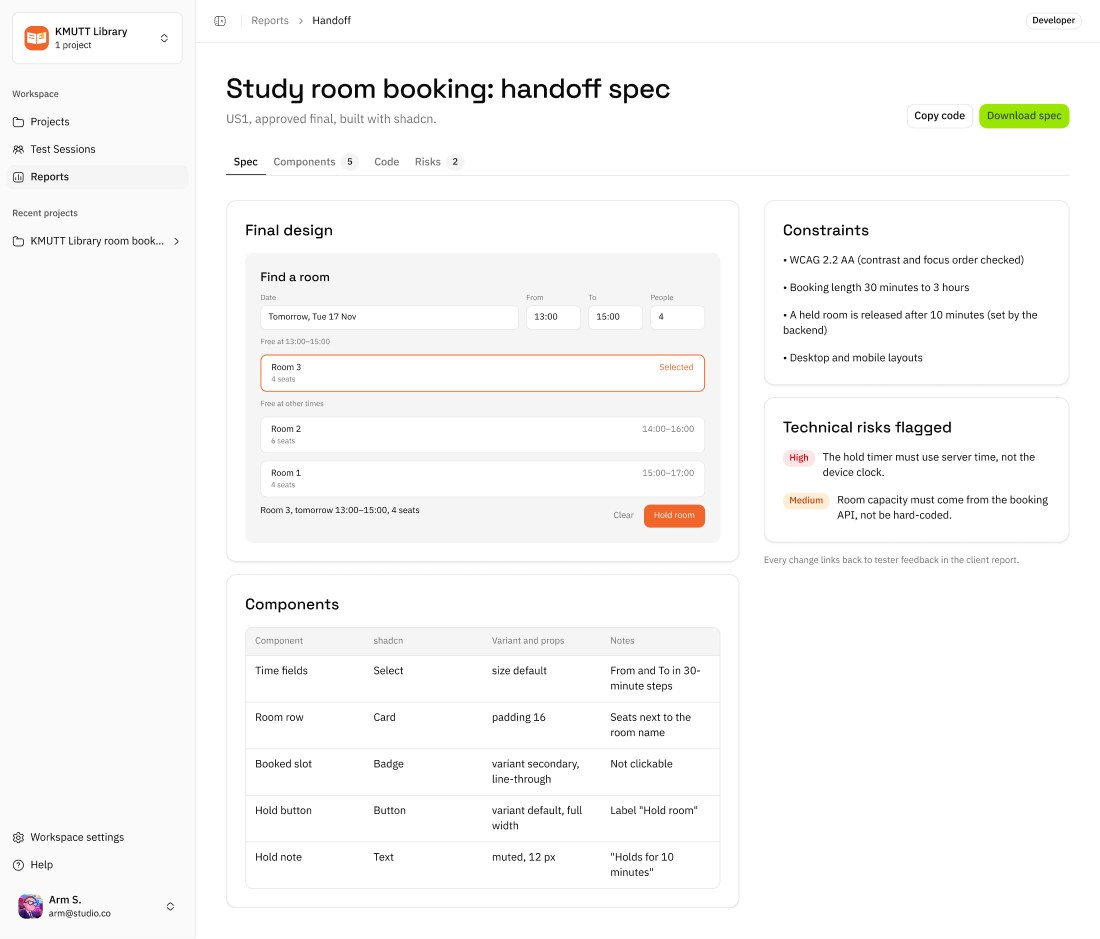
\includegraphics[width=0.48\linewidth,height=7cm,keepaspectratio]{figures/ch3-methodology/ui/s38-developer.jpg}}\\
  \subfloat[39 PM round progress]{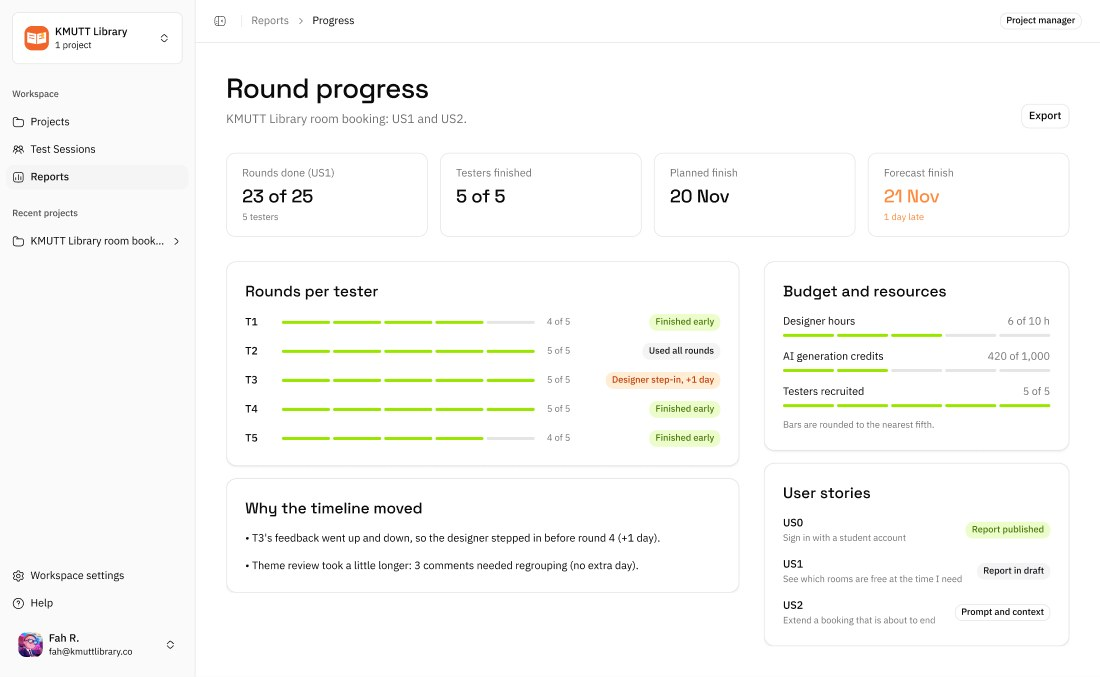
\includegraphics[width=0.48\linewidth,height=7cm,keepaspectratio]{figures/ch3-methodology/ui/s39-pm.jpg}}\\
  \caption{Prototype ของ Client, Developer และ Project Manager}
  \label{fig:ui-stakeholder}
\end{figure}
